\documentclass[conference]{IEEEtran}
\IEEEoverridecommandlockouts

\usepackage{cite}
\usepackage{newtxtext,newtxmath}
\usepackage{amsmath,amssymb}
\usepackage{graphicx}
\usepackage{booktabs}
\usepackage{multirow}
\usepackage{xcolor}
\usepackage{url}
\usepackage{algorithm}
\usepackage{algpseudocode}
\usepackage{tikz}
\usetikzlibrary{positioning,arrows.meta,fit,backgrounds,calc,shapes.geometric}
\usepackage[hidelinks]{hyperref}

% Results not yet available are shown in red so they cannot be mistaken for measurements.
\newcommand{\tbd}{\textcolor{red}{TBD}}
\newcommand{\todo}[1]{\textcolor{red}{[TODO: #1]}}
\newcommand{\yes}{\checkmark}
\newcommand{\partly}{$\circ$}
\newcommand{\no}{--}
% Includes an image if the file exists, otherwise prints a small placeholder so missing screenshots do not break layout.
\newcommand{\safeimg}[2]{\IfFileExists{#2}{\includegraphics[#1]{#2}}{\fbox{\parbox{0.9\linewidth}{\centering\footnotesize
  Missing image: \texttt{\detokenize{#2}}}}}}

% Shared diagram colours: blue = language model, orange = deterministic rule, grey = data store.
\colorlet{llmfill}{blue!7}\colorlet{llmdraw}{blue!55!black}
\colorlet{detfill}{orange!10}\colorlet{detdraw}{orange!75!black}
\colorlet{stofill}{gray!12}\colorlet{stodraw}{gray!60!black}

\begin{document}

\title{A Policy-Grounded Agentic Framework for Multi-Stakeholder Enterprise Grievance Redressal}

\author{
\IEEEauthorblockN{Dr. Bahubali Shrigarpur}
\IEEEauthorblockA{\textit{Dept. of CSE (AI \& ML)} \\
\textit{Dayananda Sagar University}\\
Bengaluru, India \\
bahubali-aiml@dsu.edu.in}
\and
\IEEEauthorblockN{Smruthi Chandrashekar}
\IEEEauthorblockA{\textit{Dept. of CSE (AI \& ML)} \\
\textit{Dayananda Sagar University}\\
Bengaluru, India \\
eng23am0281@dsu.edu.in}
\and
\IEEEauthorblockN{Y. Teja}
\IEEEauthorblockA{\textit{Dept. of CSE (AI \& ML)} \\
\textit{Dayananda Sagar University}\\
Bengaluru, India \\
eng23am0090@dsu.edu.in}
\and
\IEEEauthorblockN{Claudia Raj}
\IEEEauthorblockA{\textit{Dept. of CSE (AI \& ML)} \\
\textit{Dayananda Sagar University}\\
Bengaluru, India \\
eng23am0095@dsu.edu.in}
}

\maketitle

\begin{abstract}
International standards ask that a grievance mechanism be accessible, predictable, transparent and able to
learn. We ask whether a language-model agent can take over grievance intake and triage without giving up these
properties, and present a framework, deployed in testing at a real-estate enterprise with six departments, that
separates the two concerns: a graph-structured agent condenses multi-turn conversations, asks clarifying questions,
classifies severity and department and answers policy questions from 41 structured company policies, while
deterministic components own a four-tier service-level escalation chain, maker--checker rejection and row-level
access for 25 staff roles. We evaluate on an audited benchmark of 7,011 complaints with familiar-topic,
held-out-topic and 205 hand-written real-style test sets. (RQ1) All 47 deterministic workflow tests pass. (RQ2)
Removing generator shortcuts (a question mark alone predicted intent with 99.5\% accuracy) raised a fine-tuned
encoder's real-style severity F1 from 17 to 68 while synthetic scores did not move. Across eleven triage
configurations, the production LLM prompts are weakest on real-style text (51.6\% routing accuracy, never predicting
Critical); a fine-tuned DistilBERT ensemble with a validation-tuned safety threshold reaches 70.7\% routing accuracy
and 70.4 severity F1 at 57\,ms per message on one CPU thread; and a cascade that hands a LoRA-fine-tuned 4B LLM's
uncertain severity calls to a zero-shot decision model cuts under-triage from 65.1\% to 12.0\%, catching 12 of 14
Critical cases. Keyword guardrails flag none of the 83 real-style high-risk cases. (RQ3) The policy retriever
places the source policy in its top four passages for 79.6\% of 988 queries, and its relevance threshold trades
abstention (18.9\%) against passing only unrelated text to the model (16.4\%).
\end{abstract}

\begin{IEEEkeywords}
grievance redressal, complaint management, LLM agents, decision models, retrieval-augmented generation,
service-level escalation, distribution shift, under-triage
\end{IEEEkeywords}

% =========================================================================================
\section{Introduction}

A grievance mechanism is how an organisation hears, investigates and answers concerns from the people its
operations affect. The UN Guiding Principles on Business and Human Rights set eight effectiveness criteria for
such mechanisms: legitimate, accessible, predictable, equitable, transparent, rights-compatible, a source of
continuous learning, and based on dialogue~\cite{ungp2011}.

Recent systems automate parts of this pipeline. Mohanraj et al.~\cite{mohanraj2025railmadad} add a fine-tuned BERT
classifier, a retrieval-augmented chatbot, Whisper voice intake and SLA-based escalation to India's Rail Madad
complaint portal, and report 95.9\% accuracy, but only for a binary emergency/non-emergency decision on social-media
posts; the chatbot is not evaluated and escalation remains the portal's manual procedure. Other work ranks
government grievances by severity~\cite{suganya2025autonomous}, jointly predicts department and urgency with a
distilled encoder~\cite{shastri2025aipca}, or answers consumer-law questions with an LLM~\cite{ganatra2025grahak}.
None of these combines conversation, policy-grounded answers, multi-level severity, department routing and
enforced deadlines, and none tests its classifier on text that differs from its training data.

A real-estate developer is a demanding setting. Its stakeholders range from office staff and site labourers to
home-buyers, shareholders and neighbouring residents; their complaints are handled by six departments under
different rules and deadlines; and a single mis-triaged harassment, safety or bribery report can carry legal
consequences. A grievance mechanism adds requirements that a general agent
does not meet: errors are asymmetric (\emph{R1}); answers must come from the company's own policies (\emph{R2});
every case needs an owner, a deadline and an audit trail (\emph{R3}); and confidential cases must be visible only to
entitled staff (\emph{R4}).

This paper asks \emph{whether a language-model agent can automate grievance intake and triage while the mechanism
keeps the properties the standards require}. Our answer is a separation of concerns: the model is used only where
language understanding is needed, and every property that the criteria make a promise about (deadlines,
escalation, approvals, access) is enforced by deterministic code. We evaluate three questions:
\begin{itemize}
\item[\textbf{RQ1}] Does the governance layer enforce the promised procedure (routing, deadlines, escalation,
      approvals) in every case?
\item[\textbf{RQ2}] Which triage model generalises to unseen topics and real-style messages, and which fails least
      often in the dangerous direction (under-triage)?
\item[\textbf{RQ3}] Are policy answers grounded in the right document, and what does refusing to answer cost?
\end{itemize}

\noindent Our contributions are:
(i) a \textbf{criteria-driven design} that assigns each requirement of the UN effectiveness criteria either to the
model or to deterministic code;
(ii) an \textbf{agentic triage workflow} with a context-sufficiency gate, clarification loop and
severity-conditioned paths (Section~\ref{sec:agent});
(iii) a \textbf{governance layer} with a four-tier SLA chain, an idempotent breach monitor, maker--checker rejection
and row-level security (Section~\ref{sec:gov});
(iv) an \textbf{audited triage benchmark} with familiar-topic, held-out-topic and hand-written test sets, and
evidence that removing generator shortcuts is what improves real-style severity triage;
(v) the first \textbf{comparison of fine-tuned encoders, decision models and LLMs for grievance triage}, measured on
routing accuracy and under-triage, with an \textbf{uncertainty-aware cascade} that cuts under-triage five-fold
(Section~\ref{sec:eval}).

% =========================================================================================
\section{Related Work}

\textbf{Automated grievance systems.} Table~\ref{tab:related} compares the closest systems. Mohanraj et
al.~\cite{mohanraj2025railmadad}, our base system, is the only prior work that combines a fine-tuned classifier, a
RAG chatbot, voice intake and SLA escalation, but it evaluates only binary emergency detection. Suganya et
al.~\cite{suganya2025autonomous} rank government grievances into high, medium and low severity from text and images
with multilingual BERT; Shastri et al.~\cite{shastri2025aipca} train a multi-task, knowledge-distilled DistilBERT
for department routing and four-level urgency; Ganatra et al.~\cite{ganatra2025grahak} build an LLM and RAG
assistant for Indian consumer grievances. These systems classify a single message or answer questions; none
converses to collect missing detail, grounds answers in the organisation's own policies, or owns a case through an
enforced escalation chain.

\textbf{Complaint classification.} Fine-tuned transformers classify telecom complaints into six categories with
92.5\% accuracy~\cite{thayumanavan2025telecom}, and a compact domain-adapted BERT reaches 0.94 F1 on four-level
defect severity at under 100M parameters~\cite{chen2025lightweight}. These studies report
accuracy on test sets drawn from the training distribution; we add held-out-topic and hand-written tests and
measure the direction of severity errors, since an under-triaged case misses its deadline.

\textbf{Policy question answering.} RAG~\cite{lewis2020rag} has been applied to policy PDFs including
tables~\cite{rahman2025policyrag}, to a university's policies and guidelines with LLaMA-3 and
ChromaDB~\cite{dayata2024carolinian}, and to a utility's complaint records with a locally hosted LLM and a
clarification fallback~\cite{putro2025energyrag}. Akkiraju et al.~\cite{akkiraju2024facts} report lessons from
enterprise RAG chatbots, including access control for HR content. RAGAs evaluates such systems
with an LLM judge; we measure retrieval directly against known source documents.

\textbf{Agents and decision models.} LLM agents interleave reasoning and action; graph
frameworks such as LangGraph make control flow explicit and have been used for multi-agent banking
assistants~\cite{easin2024langgraph}. We borrow clarifying questions and query
rewriting from conversational search. A recent class of \emph{decision models} returns a
probability for every option of a typed question instead of generating text~\cite{cloudflare2026clef,convai2026laya}, which suits routing; we compare them with fine-tuned encoders and
LoRA-fine-tuned LLMs.


\begin{table}[t]
\centering
\caption{Comparison with the closest grievance systems. \yes: present and evaluated; \part: present but not
evaluated; \no: absent.}
\label{tab:related}
\footnotesize
\setlength{\tabcolsep}{2.4pt}
\begin{tabular}{@{}lccccc@{}}
\toprule
 & Rail Madad & Govt. & AIPCA & Grahak- & \textbf{This} \\
 & \cite{mohanraj2025railmadad} & \cite{suganya2025autonomous} & \cite{shastri2025aipca} & Nyay~\cite{ganatra2025grahak} & \textbf{work} \\
\midrule
Severity levels           & 2 & 3 & 4 & \no & 3--4 \\
Department routing        & \partly & \yes & \yes & \no & \yes \\
Clarifying dialogue       & \no & \no & \no & \yes & \yes \\
Policy-grounded answers   & \partly & \no & \no & \yes & \yes \\
Enforced SLA escalation   & \partly & \no & \partly & \no & \yes \\
Voice / multilingual      & \yes & \yes & \yes & \partly & \yes \\
Real-style / OOD test     & \no & \no & \no & \partly & \yes \\
Under-triage measured     & \no & \no & \no & \no & \yes \\
Encoder vs.\ LLM compared & \no & \no & \partly & \no & \yes \\
\bottomrule
\end{tabular}
\end{table}

% =========================================================================================
\section{System Architecture}

Fig.~\ref{fig:arch} shows the five layers of the framework. Complainants and staff use a progressive web
application built with React; voice is transcribed with Whisper and user text is
translated on the server while labels, statuses and identifiers are never translated. A FastAPI service hosts the
agent, the knowledge layer and the governance services, and PostgreSQL (Supabase) stores grievances, escalation
history, notifications and audit logs and pushes real-time updates to dashboards. The triage classifier is
swappable: the deployed system calls a hosted LLM (Qwen3 27B on Groq), and Section~\ref{sec:models} evaluates
local replacements.

\begin{figure*}[t]
\centering
\resizebox{\textwidth}{!}{%
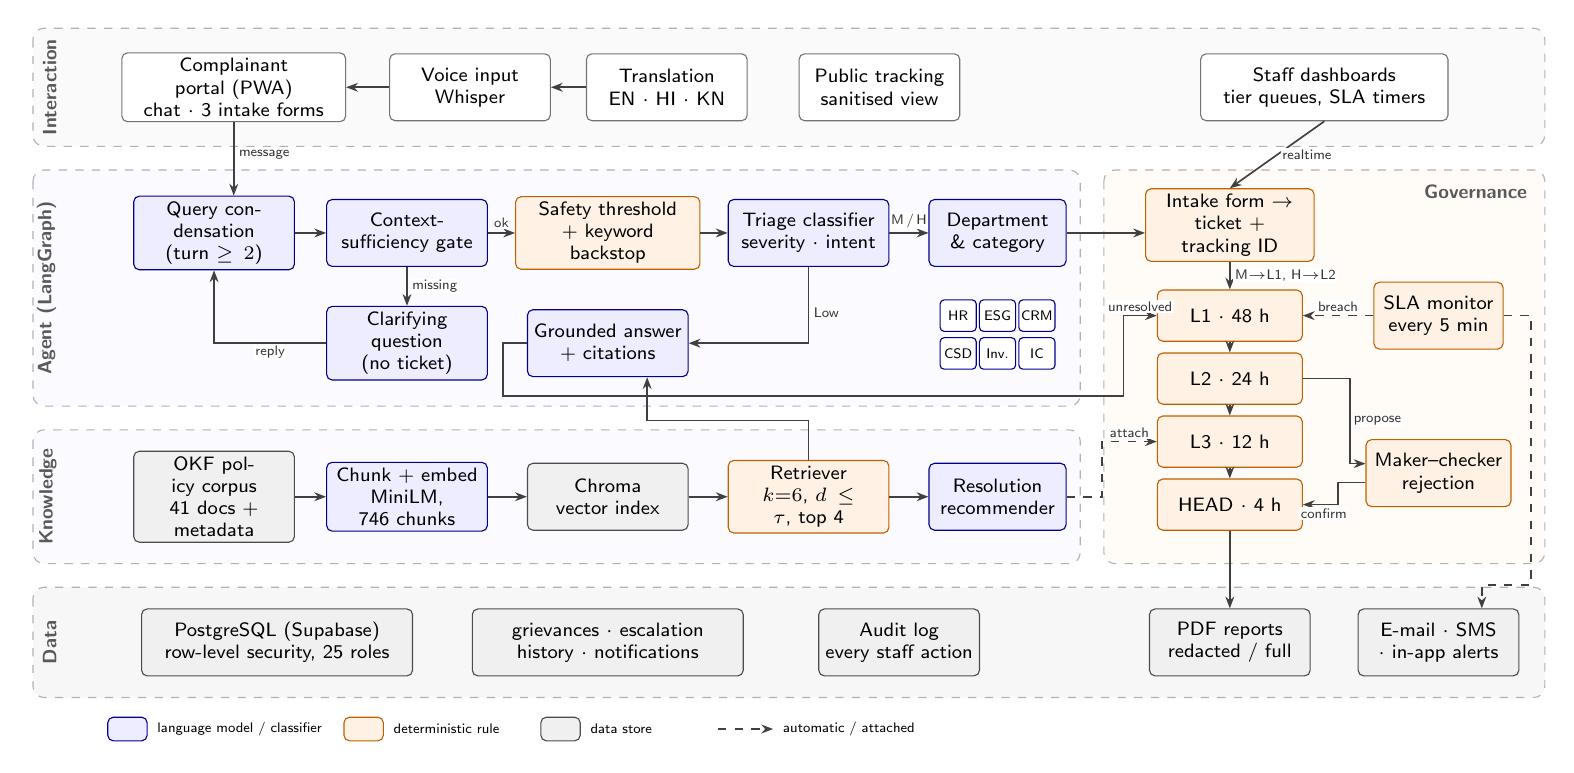
\begin{tikzpicture}[
  font=\sffamily\scriptsize,
  node distance=4mm,
  base/.style={draw, rounded corners=2pt, align=center, minimum height=8.5mm, inner sep=2pt},
  llm/.style={base, fill=llmfill, draw=llmdraw, text width=#1}, llm/.default=19mm,
  det/.style={base, fill=detfill, draw=detdraw, text width=#1}, det/.default=19mm,
  sto/.style={base, fill=stofill, draw=stodraw, text width=#1}, sto/.default=19mm,
  ui/.style={base, fill=white, draw=black!55, text width=#1}, ui/.default=19mm,
  tier/.style={base, fill=detfill, draw=detdraw, text width=17mm, minimum height=6.5mm},
  chip/.style={draw=llmdraw, fill=white, rounded corners=1.5pt, font=\sffamily\tiny, minimum width=8mm,
               minimum height=4mm, inner sep=0.5pt},
  band/.style={draw=black!30, dashed, rounded corners=4pt, fill=#1},
  lane/.style={font=\sffamily\scriptsize\bfseries, text=black!65, rotate=90, anchor=south},
  arr/.style={-{Stealth[length=1.5mm]}, semithick, black!75},
  dar/.style={arr, dashed},
  lbl/.style={font=\sffamily\tiny, fill=white, inner sep=0.6pt, text=black!80},
]
% ---------- bands ----------
\draw[band=black!2]  (0,0.75) rectangle (19.2,-0.75);
\draw[band=blue!2]   (0,-1.05) rectangle (13.3,-4.05);
\draw[band=blue!2]   (0,-4.35) rectangle (13.3,-6.05);
\draw[band=orange!3] (13.6,-1.05) rectangle (19.2,-6.05);
\draw[band=black!3]  (0,-6.35) rectangle (19.2,-7.75);
\node[lane] at (0.42,0)     {Interaction};
\node[lane] at (0.42,-2.55) {Agent (LangGraph)};
\node[lane] at (0.42,-5.2)  {Knowledge};
\node[lane] at (0.42,-7.05) {Data};
\node[font=\sffamily\scriptsize\bfseries, text=black!65, anchor=north east] at (19.1,-1.12) {Governance};

% ---------- interaction ----------
\node[ui=27mm] (portal) at (2.55,0)  {Complainant portal (PWA)\\chat $\cdot$ 3 intake forms};
\node[ui]      (voice)  at (5.55,0)  {Voice input\\Whisper};
\node[ui]      (trans)  at (8.05,0)  {Translation\\EN $\cdot$ HI $\cdot$ KN};
\node[ui]      (track)  at (10.75,0) {Public tracking\\sanitised view};
\node[ui=30mm] (dash)   at (16.4,0)  {Staff dashboards\\tier queues, SLA timers};
\draw[arr] (voice) -- (portal);
\draw[arr] (trans) -- (voice);

% ---------- agent ----------
\node[llm] (cond) at (2.3,-1.85)  {Query condensation\\(turn $\geq 2$)};
\node[llm] (ctx)  at (4.75,-1.85) {Context-\\sufficiency gate};
\node[det=22mm] (grd) at (7.3,-1.85) {Safety threshold\\+ keyword backstop};
\node[llm] (sev)  at (9.85,-1.85) {Triage classifier\\severity $\cdot$ intent};
\node[llm] (clar) at (4.75,-3.25) {Clarifying question\\(no ticket)};
\node[llm] (ans)  at (7.3,-3.25)  {Grounded answer\\+ citations};
\node[llm=16mm] (dep) at (12.25,-1.85) {Department\\\& category};
\foreach \d/\x/\y in {HR/11.75/-2.9, ESG/12.25/-2.9, CRM/12.75/-2.9, CSD/11.75/-3.38, Inv./12.25/-3.38, IC/12.75/-3.38}
  \node[chip, minimum width=4.6mm] at (\x,\y) {\d};

\draw[arr] (portal.south) -- node[lbl, right=1pt, pos=0.45]{message} (portal.south |- cond.north);
\draw[arr] (cond) -- (ctx);
\draw[arr] (ctx) -- node[lbl, above=1pt]{ok} (grd);
\draw[arr] (grd) -- (sev);
\draw[arr] (sev) -- node[lbl, above=1pt]{M\,/\,H} (dep);
\draw[arr] (ctx) -- node[lbl, right=1pt]{missing} (clar);
\draw[arr] (clar.west) -| node[lbl, pos=0.25, below]{reply} (cond.south);
\draw[arr] (sev.south) |- node[lbl, pos=0.3, right=1pt]{Low} (ans.east);

% ---------- knowledge ----------
\node[sto] (okf)  at (2.3,-5.2)  {OKF policy corpus\\41 docs + metadata};
\node[llm] (emb)  at (4.75,-5.2) {Chunk + embed\\MiniLM, 746 chunks};
\node[sto] (idx)  at (7.3,-5.2)  {Chroma\\vector index};
\node[det] (retr) at (9.85,-5.2) {Retriever\\$k{=}6$, $d \leq \tau$, top 4};
\node[llm=16mm] (rec) at (12.25,-5.2) {Resolution\\recommender};
\draw[arr] (okf) -- (emb);
\draw[arr] (emb) -- (idx);
\draw[arr] (idx) -- (retr);
\draw[arr] (retr.north) -- ++(0,0.5) -| ($(ans.south)+(0.5,0)$);
\draw[arr] (retr) -- (rec);

% ---------- governance ----------
\node[det] (tkt) at (15.2,-1.75) [text width=20mm] {Intake form $\rightarrow$\\ticket + tracking ID};
\node[tier] (l1) at (15.2,-2.9)  {L1 $\cdot$ 48 h};
\node[tier] (l2) at (15.2,-3.7)  {L2 $\cdot$ 24 h};
\node[tier] (l3) at (15.2,-4.5)  {L3 $\cdot$ 12 h};
\node[tier] (hd) at (15.2,-5.3)  {HEAD $\cdot$ 4 h};
\node[det] (sla) at (17.85,-2.9) [text width=15mm] {SLA monitor\\every 5 min};
\node[det] (mc)  at (17.85,-4.9) [text width=17mm] {Maker--checker\\rejection};
\draw[arr] (dep.east) -- (tkt.west |- dep.east);
\draw[arr] (tkt) -- node[lbl, right=1pt]{M$\to$L1, H$\to$L2} (l1);
\draw[arr] (l1) -- (l2);
\draw[arr] (l2) -- (l3);
\draw[arr] (l3) -- (hd);
\draw[dar] (sla.west) -- node[lbl, above=0.5pt]{breach} (l1.east);
\draw[arr] (l2.east) -- ++(0.6,0) |- node[lbl, pos=0.25, right=0.5pt]{propose} ($(mc.west)+(0,0.12)$);
\draw[arr] ($(mc.west)+(0,-0.12)$) -- ++(-0.35,0) |- node[lbl, pos=0.7, below=0.5pt]{confirm} (hd.east);
\draw[arr] (ans.west) -- ++(-0.3,0) |- (13.85,-3.92) |- node[lbl, pos=0.75, above=0.5pt]{unresolved} (l1.west);
\draw[dar] (rec.east) -- ++(0.45,0) |- node[lbl, pos=0.75, above=0.5pt]{attach} (l3.west);
\draw[arr] (dash.south) -- node[lbl, right=1pt]{realtime} (tkt.north);

% ---------- data ----------
\node[sto=33mm] (db)    at (3.1,-7.05)  {PostgreSQL (Supabase)\\row-level security, 25 roles};
\node[sto=33mm] (tabs)  at (7.3,-7.05)  {grievances $\cdot$ escalation\\history $\cdot$ notifications};
\node[sto]      (audit) at (11.0,-7.05) {Audit log\\every staff action};
\node[sto]      (pdf)   at (15.2,-7.05) {PDF reports\\redacted / full};
\node[sto=19mm] (notif) at (17.85,-7.05) {E-mail $\cdot$ SMS\\$\cdot$ in-app alerts};
\draw[arr] (hd.south) -- (pdf.north);
\draw[dar] (sla.east) -- ++(0.35,0) |- ($(notif.north)+(0.55,0.3)$) -- ($(notif.north)+(0.55,0)$);

% ---------- legend ----------
\node[base, fill=llmfill, draw=llmdraw, minimum height=3mm, minimum width=5mm] (k1) at (1.2,-8.15) {};
\node[anchor=west, font=\sffamily\tiny] at (k1.east) {language model / classifier};
\node[base, fill=detfill, draw=detdraw, minimum height=3mm, minimum width=5mm] (k2) at (4.2,-8.15) {};
\node[anchor=west, font=\sffamily\tiny] at (k2.east) {deterministic rule};
\node[base, fill=stofill, draw=stodraw, minimum height=3mm, minimum width=5mm] (k3) at (6.7,-8.15) {};
\node[anchor=west, font=\sffamily\tiny] at (k3.east) {data store};
\draw[dar] (8.7,-8.15) -- (9.4,-8.15) node[anchor=west, font=\sffamily\tiny, text=black] {automatic / attached};
\end{tikzpicture}}%
\caption{Layered architecture. The agent (blue) decides between a grounded self-service answer and human handling;
the governance column (orange) owns tickets, tiers, deadlines and approvals; everything is persisted under
row-level security. The triage classifier is the LLM in deployment and is replaceable by the models of
Section~\ref{sec:models}. M\,/\,H: medium or high severity; $\tau$: relevance threshold.}
\label{fig:arch}
\end{figure*}

% =========================================================================================
\section{Agentic Triage Workflow}
\label{sec:agent}

The agent is a typed state graph with nine nodes. An explicit control
flow, rather than free tool choice, keeps every path to a ticket inspectable and testable; in
this sense the agent is an LLM-orchestrated workflow~\cite{easin2024langgraph} rather than an autonomous planner.

\textbf{Condensation.} A follow-up such as ``Tower B, 402'' is meaningless alone. From the second turn on, an LLM
rewrites the latest message, recent history and answers to clarifying questions into one stand-alone
statement, resolving pronouns and dropping topics the user has left. The first turn
bypasses the model, so single-message complaints incur no extra latency.

\textbf{Context sufficiency.} Policy questions pass immediately. For grievances the agent judges whether enough
operational detail (location, project, time, amount) has been given to route the case; if not, it asks one
targeted question~\cite{putro2025energyrag} and creates no ticket and no deadline.
Harassment, physical danger and bribery reports are always treated as sufficient, so urgent cases are never delayed
by a question.

\textbf{Severity and safety.} The classifier assigns intent and severity; policy questions are always low severity,
and an unparseable output falls back to a safe default and is logged. Because missing a serious case is worse than
over-escalating a routine one (R1), the final severity is not the classifier's arg-max: a case is escalated to High
when the predicted probability of High or Critical exceeds a threshold tuned on validation data, and in the
cascade variant uncertain calls are re-asked of a second model (Algorithm~\ref{alg:sev}). Deterministic keyword
rules for harassment, site-safety and fraud remain as a backstop for explicit wording.

\textbf{Two paths.} Low-severity messages go to policy retrieval and a grounded answer (Section~\ref{sec:rag}); if
the user is still unsatisfied, the conversation is handed to an L1 officer with the transcript. Medium- and
high-severity grievances are classified into one of six departments and a fixed list of categories (e.g.,
\emph{Possession \& Handover} for CRM); the complainant confirms the case in a structured form, which creates the
ticket and returns a tracking identifier.

\begin{algorithm}[t]
\caption{Uncertainty-aware severity decision}
\label{alg:sev}
\footnotesize
\begin{algorithmic}[1]
\Require message $x$; primary model $f$; fallback decision model $g$; thresholds $\theta$, $\gamma$ (validation)
\State $p \gets f(x)$ \Comment{probabilities over Low, Medium, High, Critical}
\State $c \gets \exp\!\big(-\sum_k p_k\,\mathrm{cost}(k)\big)$ \Comment{under-triage costs 2 per level, over-triage 1}
\If{cascade enabled \textbf{and} $c < \gamma$} $p \gets g(x)$ \Comment{$\gamma = 0.593$}
\EndIf
\State $s \gets \arg\max_k p_k$
\If{$s < \mathrm{High}$ \textbf{and} $p_{\mathrm{High}} + p_{\mathrm{Critical}} \geq \theta$} $s \gets \mathrm{High}$
\EndIf
\If{keyword rule fires \textbf{and} $x$ is not a question} $s \gets \max(s, \mathrm{High})$
\EndIf
\State \Return $s$ \Comment{Low $\to$ RAG; Medium $\to$ L1; High/Critical $\to$ L2}
\end{algorithmic}
\end{algorithm}
% =========================================================================================
\section{Governance Layer}
\label{sec:gov}

\textbf{Tiers and deadlines.} Each department has four tiers, L1, L2, L3 and HEAD, with SLAs of 48, 24, 12 and
4 hours. Medium-severity cases start at L1 and high-severity cases at L2. A background
monitor (Algorithm~\ref{alg:sla}) moves a breached case one tier up, resets its deadline, appends to its
escalation history and notifies the complainant and department. It checks the last recorded transition before
writing, so a restart or an overlapping run never escalates a case twice. Unlike the manual escalation matrix of
the base system~\cite{mohanraj2025railmadad}, no human action is needed for a case to move up. High- and
critical-severity cases additionally trigger e-mail and SMS alerts, with contacts looked up from the database
rather than configuration.

\begin{algorithm}[t]
\caption{SLA monitor (runs every 5 minutes)}
\label{alg:sla}
\footnotesize
\begin{algorithmic}[1]
\State $\mathit{SLA} \gets \{\mathrm{L1}{:}48, \mathrm{L2}{:}24, \mathrm{L3}{:}12, \mathrm{HEAD}{:}4\}$ hours
\For{each case $c$ in human handling with $c.\mathit{deadline} < \mathit{now}$}
  \If{$c.\mathit{tier} = \mathrm{HEAD}$} \textbf{continue} \Comment{ceiling}
  \EndIf
  \State $t' \gets \textsc{Next}(c.\mathit{tier})$ \Comment{L1$\to$L2$\to$L3$\to$HEAD}
  \If{last entry of $c.\mathit{history}$ already moved to $t'$} \textbf{continue}
  \EndIf
  \State append $(c.\mathit{tier} \to t', \textsc{SlaBreach}, \mathit{now})$ to $c.\mathit{history}$
  \State $c.\mathit{tier} \gets t'$;\; $c.\mathit{deadline} \gets \mathit{now} + \mathit{SLA}[t']$
  \State notify complainant and department staff of tier $t'$
\EndFor
\end{algorithmic}
\end{algorithm}

\textbf{Maker--checker rejection.} Closing a complaint as invalid is the most sensitive staff action. L1--L3
officers may only \emph{propose} a rejection, which routes the case to HEAD; HEAD (or a super-administrator)
confirms it or returns the case to the proposing tier. Only HEAD can reject directly.

\textbf{Access control and accountability.} Staff roles are the 24 combinations of six departments and four tiers
plus one super-administrator; everyone else is a complainant. Row-level security policies
restrict each table to the rows a role may see, the service credential that bypasses them never leaves the server,
and every administrative action is written to an audit log. Accounts are tied to a verified phone number to deter
mass fake submissions, anonymous reports are tracked only by an unguessable identifier, and each case can be
exported as a redacted PDF for the complainant or a full one for HEAD.

% =========================================================================================
\section{Policy Knowledge Layer}
\label{sec:rag}

The company's 41 policies (POSH, whistle-blower, anti-bribery, leave, relocation, CSR, materiality, dividend,
related-party transactions and others), eight of them scanned and converted with OCR, are converted to Markdown with
machine-readable front matter following the Open Knowledge Format: owning department, target stakeholder groups,
document type (policy, procedure, escalation matrix, FAQ), authority and version. As in other policy-document
assistants~\cite{rahman2025policyrag,dayata2024carolinian}, documents are split into 1,000-character chunks with 200
characters of overlap (746 chunks), embedded with MiniLM and stored in a
Chroma index; each chunk keeps its metadata so answers can cite the policy and section.

At query time the agent rewrites follow-up questions into stand-alone queries, retrieves six chunks, removes
duplicates, discards chunks whose distance exceeds a relevance threshold $\tau$ and passes at most four to the
model. If nothing passes, the assistant states that the question is not covered rather than
improvising~\cite{akkiraju2024facts}, and generated answers are post-processed to remove contact details that do
not come from the sources. The same index powers a staff-facing \emph{resolution recommender}: when a high-severity
or policy-related case is assigned, matching clauses are summarised into procedural steps and compliance checks
attached to the ticket.

% =========================================================================================
\section{Evaluation}
\label{sec:eval}

\subsection{RQ1: Workflow correctness}
Deterministic behaviour is covered by 47 unit tests that run without network access, and all pass: 35 for
routing and SLAs (severity normalisation, initial tier and deadline for every severity--department pair, chatbot
hand-off, the full escalation chain including the HEAD ceiling), 9 for maker--checker rejection (propose,
confirm, overturn, direct reject) and 3 for multi-turn condensation followed by correct routing. Because these
behaviours are rules, the tests can enumerate their input space instead of sampling it.

\subsection{RQ2: Triage under topic shift and real-style text}
\label{sec:bench}

\textbf{Benchmark.} Real complaints are confidential, so the benchmark was generated with three LLMs from company
seed material (HR issue lists, CRM project logs, a customer-service concerns workbook, ESG stakeholder registers
with category A/B/C severity definitions, and 32 policies): 8,360 records labelled with
department, severity (Low/Medium/High/Critical) and intent, 7,302 after exact deduplication. An audit of this first
version found that it could be solved from surface cues: a trailing question mark
predicted intent with 99.5\% accuracy, urgency words appeared in 42.9\% of Critical but 0.9\% of Low complaints,
2,332 policy questions had a severity above Low, and 703 bribery and misconduct reports were filed under the
harassment committee. The released version (v2) restyles 3,148 rows (question and statement
forms, typos, Hinglish, no politeness), removes urgency cues from half of the Critical rows, makes every policy
question Low, re-routes non-harassment IC rows to the department they concern, and adds 263 hand-written training
and validation messages. It has 7,011 rows in 5,754 scenario groups. Every group stays in one split, and 17 whole
topics are held out as an unseen-topic test set (\texttt{OOD}). A separate set of 205 hand-written, real-style
messages (\texttt{Real}: 160 grievances, 45 queries, 14 Critical) is never used for training or prompting. Version
v2.1 adds 112 hand-written severity rows (45 Critical hazards described plainly, 35 Low, 32 Medium/High boundary
pairs) to training and validation only; all test files are unchanged. Severity is scored on grievances only, since
every policy question is Low by construction.
\textbf{Leakage and shortcuts.} After the audit, the question-mark rule drops from 99.5\%
to 73.7\% intent accuracy. Copying the label of the nearest training message (MiniLM cosine) reaches 85.9
department F1 under a random re-split, where 14.9\% of test rows have a training paraphrase ($\geq$0.85); under our
splits only 0.2--2.4\% do, and copying falls to 67.0 on unseen topics. Training the same TF-IDF + logistic
regression recipe on the audited data instead of the original raises real-style department F1 from 81.4 to 86.8 and
grievance severity F1 from 24.4 to 33.6. The effect is larger for a fine-tuned encoder (Fig.~\ref{fig:gap}):
DistilBERT trained on the synthetic rows alone scores 69.2 four-level severity F1 on familiar topics but 17.4 on
real-style text; adding the hand-written rows raises the real-style score to 54.2 (v2) and 67.5 (v2.1, with the
decision layer) while the synthetic score stays near 70, so a synthetic test set alone would have hidden both the
failure and the fix. After the audit, the DistilBERT models lose only 4--6 mean-F1 points from familiar topics to
real-style text, against 9 for TF-IDF (Fig.~\ref{fig:gap}).
\begin{figure}[t]
\centering
\safeimg{width=\columnwidth}{figures/synthetic_vs_real_gap.jpg}
\caption{Mean macro-F1 (department, severity, intent) of the baselines and DistilBERT variants on familiar-topic,
unseen-topic and real-style test sets, trained on v2.1. A steep drop would indicate overfitting to the generator's
style.}
\label{fig:gap}
\end{figure}

\subsection{Triage models}
\label{sec:models}

We compare five families on identical splits and metrics (Table~\ref{tab:models}).
\emph{Baselines}: keyword rules and TF-IDF + logistic regression.
\emph{Production LLM}: the deployed prompts and guardrails, two calls per message to Qwen3 27B on Groq at
temperature zero. \emph{Decision models}~\cite{cloudflare2026clef,convai2026laya}: Clef-flash 9B (4-bit, local),
one call answering department, severity and intent, with department definitions copied from the production prompt
(v1) or derived from the training split (v2); and Laya, a 421M ModernBERT-large decision model, zero-shot and
fine-tuned. \emph{Fine-tuned encoder}: multi-task DistilBERT with one head per task,
in the spirit of~\cite{shastri2025aipca,chen2025lightweight}. \emph{Fine-tuned LLM}: Qwen3-4B-Instruct with LoRA
adapters, which scores every allowed label instead of generating free text, so every row receives
a valid label. On top of the probabilistic models we tune a \emph{decision layer} on validation only: a per-class
severity bias, the safety threshold $\theta$ of Algorithm~\ref{alg:sev} (minimising $3\times$under-triage $+$
over-triage), and, for the fine-tuned LLM, the cascade hand-off $\gamma$ to Clef-flash.

\begin{table}[t]
\centering
\caption{Triage models and training. All fine-tuning ran on one T4 GPU; tuning used validation data only.}
\label{tab:models}
\footnotesize
\setlength{\tabcolsep}{2.5pt}
\begin{tabular}{@{}lp{5.6cm}@{}}
\toprule
Model & Configuration \\
\midrule
DistilBERT & 66M; 3 linear heads on [CLS]; class-weighted CE ($\propto$count$^{-0.5}$), label smoothing 0.1; AdamW,
lr $5{\cdot}10^{-5}$, 10 epochs, patience 3, batch 32, fp16; 5 seeds; v2.1 train \\
Laya (FT) & 421M ModernBERT-large; \texttt{laya.train.finetune}, 3 epochs, batch $8{\times}8$, encoder lr
$2.5{\cdot}10^{-5}$, head lr $10^{-4}$, option shuffling; 11,645 training questions; v2.1 train \\
Qwen3-4B (FT) & LoRA $r{=}16$, $\alpha{=}32$ on all attention and MLP projections; loss on the answer only;
1 epoch, lr $2{\cdot}10^{-4}$, effective batch 8; v2 train \\
Clef-flash 9B & zero-shot; 4-bit MLX weights; one call per message \\
Production LLM & zero-shot; Qwen3 27B (Groq); 2 calls; keyword guardrails on \\
\bottomrule
\end{tabular}
\end{table}

\begin{table*}[t]
\centering
\caption{Triage results (\%) for the best configuration in each model family (all configurations in
Fig.~\ref{fig:triage}). Department: macro-F1 on hand-written (Real), familiar-topic (ID) and unseen-topic (OOD)
test sets. Severity: 3-level macro-F1 on the 160 real-style grievances (Critical merged into High, as in routing).
Routing: department and tier both correct. Under-triage: share of cases that belong in L2 but are sent to L1 or
the chatbot; over-triage: share of the rest sent higher. 95\% bootstrap intervals in brackets. ZS: zero-shot; FT:
fine-tuned. $^\dagger$trained on v2.1, otherwise v2. $^\ddagger$159 of 205 rows (rate-limited).}
\label{tab:triage}
\footnotesize
\setlength{\tabcolsep}{4pt}
\begin{tabular}{@{}llccccccc@{}}
\toprule
 & & \multicolumn{3}{c}{Department F1} & Severity F1 & Routing & Under- & Over- \\
\cmidrule(lr){3-5}
Family & Model & Real & ID & OOD & Real & acc.\ Real & triage $\downarrow$ & triage $\downarrow$ \\
\midrule
Baseline & TF-IDF + LR & 86.8 & 91.4 & 78.3 & 43.3 & 56.1 & 54.2 & \textbf{11.5} \\
LLM (ZS) & Production prompts, Qwen3 27B$^\ddagger$ & 54.6 & -- & -- & 47.4 & 51.6 & 50.9 & \textbf{11.5} \\
Decision model (ZS) & Clef-flash 9B & 90.2 & 82.4 & 81.8 & 55.1 & 70.2 & 14.5 & 26.2 \\
Encoder (FT) & DistilBERT ensemble + bias + $\theta$$^\dagger$ & 87.9 & \textbf{92.9} & 84.2 & \textbf{70.4} & \textbf{70.7} [64.4, 76.6] & 19.3 [10.8, 27.5] & 20.5 \\
LLM (FT) & Cascade: Qwen3-4B LoRA $\to$ Clef-flash & \textbf{91.1} & 92.4 & \textbf{86.8} & 65.0 & 69.8 [63.9, 76.1] & \textbf{12.0} [5.9, 19.4] & 34.4 \\
\bottomrule
\end{tabular}
\end{table*}

\begin{figure*}[t]
\centering
\safeimg{width=0.82\textwidth}{figures/model_comparison.png}
\caption{Department F1, severity F1 and routing accuracy of all eleven evaluated configurations on the 205
hand-written messages. Colour: grey baseline, blue LLM, orange decision model, green fine-tuned encoder, purple
cascade.}
\label{fig:triage}
\end{figure*}

\textbf{Main result.} Table~\ref{tab:triage} and Fig.~\ref{fig:triage} answer RQ2. (1) \emph{The deployed LLM
prompts are the weakest probabilistic option}: 54.6 department F1 and 51.6\% routing accuracy, no Critical
predictions, no probabilities for a review threshold, and 31 of 159 messages without a valid department. (2)
\emph{Department routing is solved by fine-tuning}: Qwen3-4B, Laya and DistilBERT all reach 88--91 F1 on real-style
text, against 42.7 for zero-shot Laya, whose option descriptions are silently truncated to about 29 tokens by its
192-token question budget. (3) \emph{Severity is the hard task}, and the fine-tuned encoder handles it best: the
DistilBERT ensemble with the decision layer reaches 70.4 severity F1 and 70.7\% routing accuracy (McNemar against
TF-IDF: severity $p{=}0.0002$, routing $p{=}0.010$). (4) \emph{Fine-tuning on synthetic data teaches its severity
style}: the LoRA model catches only 3 of 14 Critical messages; 11 of them describe a live hazard calmly (an
uncovered well where children play, a crane under a sagging 66\,kV line), whereas synthetic Critical rows used
urgency words. (5) \emph{Zero-shot severity is safe but blunt}: Clef-flash catches all 14 Critical messages and has
the lowest under-triage (6.0\%) but over-escalates a third of the rest. (6) \emph{Combining them works}: the cascade
keeps the fine-tune's department routing and hands its uncertain severity calls to Clef-flash, cutting under-triage
from 65.1\% to 12.0\% (non-overlapping intervals) and catching 12 of 14 Critical cases; its routing gain is
borderline ($p{=}0.056$). The fine-tune hands off 60\% of real-style but only about 30\% of synthetic messages, so a
threshold tuned on validation transfers to the text where it is needed.

\textbf{Generalisation and error structure.} Every supervised model loses 6--13 department F1 points from familiar
to unseen topics (Table~\ref{tab:triage}), the TF-IDF baseline most, consistent with the shift sensitivity of
lexical models; zero-shot Clef-flash is the most stable (82.4 to 81.8). On synthetic test
sets the ranking flips: the LoRA model with a safety threshold is best on every column, so \emph{a model chosen on
synthetic scores alone would ship the one that misses 11 of 14 Critical messages}. The most consequential routing
error is Internal Committee (harassment) cases sent to HR: 24\% for the TF-IDF baseline and 18\% for fine-tuned
Laya on real-style text. A harassment report that reaches a line HR officer loses the confidentiality the law
requires.
\textbf{Confidence and the safety threshold.} Temperature scaling lowers DistilBERT's expected calibration error
for department (7.5 to 5.5), severity (11.3 to 9.0) and intent (3.1 to 2.7); the LoRA model is already calibrated
(department ECE 5.1) and scaling on the mostly synthetic validation set makes its severity worse. Fine-tuned Laya's
fitted temperature hits the library's upper clamp, a sign of over-confidence on training-like text. The safety
threshold roughly halves under-triage for every model it is applied to (DistilBERT 36.1 to 19.3, Laya 49.4 to 25.3,
Qwen3-4B 65.1 to 34.9) at the cost of more over-triage (Fig.~\ref{fig:thr}); since an over-triaged case only
reaches a senior officer early, we accept this trade.

\begin{figure}[t]
\centering
\safeimg{width=\columnwidth}{figures/severity_threshold.jpg}
\caption{Effect of the severity safety threshold $\theta$ on real-style messages (single DistilBERT model; the
dashed line marks $\theta{=}0.2$ chosen on validation). Lowering $\theta$ trades under-triage for over-triage while
routing accuracy stays flat until $\theta \approx 0.1$.}
\label{fig:thr}
\end{figure}

\textbf{Guardrails.} The deterministic keyword rules were meant to catch exactly these cases. They fire on none of
the 83 real-style High and Critical grievances; on the real-style set they fired four times and were wrong every
time, twice on policy questions (``how can a vendor report a bribe demand anonymously'') and twice on Medium
harassment follow-ups. Adding them to DistilBERT lowers routing accuracy from 66.0\% to 64.6\%. Keyword rules are
therefore a backstop for explicit wording, not a safety net; protection against under-triage comes from the
calibrated threshold and the cascade.

\textbf{Efficiency.} Table~\ref{tab:eff} shows the cost of each option. DistilBERT runs in 57\,ms per message on
one CPU thread (23\,ms quantised to int8 at a 3.9-point loss in mean F1) with no per-call cost or rate limit; the
local decision model and LoRA model need about one second, and the hosted production LLM 14\,s at the median,
dominated by free-tier rate-limit waits.

\begin{table}[t]
\centering
\caption{Inference cost per message (median). Hardware differs, so figures are indicative.}
\label{tab:eff}
\footnotesize
\setlength{\tabcolsep}{3pt}
\begin{tabular}{@{}lrll@{}}
\toprule
Model & Size & Hardware & Latency \\
\midrule
TF-IDF + LR & small & CPU & 0.5\,ms \\
DistilBERT fp32 & 266\,MB & CPU, 1 thread & 57\,ms \\
DistilBERT int8 & 138\,MB & CPU, 1 thread & 23\,ms \\
DistilBERT fp32 & 266\,MB & T4 GPU & 4.6\,ms \\
Clef-flash 9B (4-bit) & 6.2\,GB & Apple M5, MLX & 975\,ms \\
Qwen3-4B + LoRA & 8\,GB + 132\,MB & T4 GPU & 1,426\,ms \\
Production LLM (2 calls) & 27B hosted & Groq cloud & 14,162\,ms \\
\bottomrule
\end{tabular}
\end{table}

\subsection{RQ3: Grounded policy answers}
To evaluate the retriever without an LLM judge, we use the 988 benchmark policy queries whose
source document is in the index and check whether the production pipeline returns a chunk of that document.
The correct policy is among the top four passages for 79.6\% of queries and first for 61.1\% (MRR 0.692). Quality
is uneven: HR, IC and Investors policies are retrieved well (82.4--85.3\% in the top four), whereas only 67.1\% of
ESG and 47.1\% of the few CRM queries are, because these concern operational procedures that are only partly
written down in the indexed policies. The deployed recommender shows the same gap: it attached a
conveyance-reimbursement form to a possession-delay complaint. The threshold $\tau$ is the main design lever. The
production value makes the assistant decline 18.9\% of queries; relaxing it to 1.15 raises grounded answers by 8.5
points but increases the cases where only unrelated passages reach the model from 16.4\% to 18.6\%. We keep the
conservative setting, since an unanswered policy question can be escalated while a confidently wrong policy answer
cannot be detected by the complainant. Retrieval takes 3.8\,ms (median) on a laptop CPU.

% =========================================================================================
\section{Discussion and Limitations}

\textbf{Lessons.} (1) \emph{Routing categories are a specification.} The first benchmark and the deployed prompt
disagreed about what the Internal Committee handles (703 rows), and changing only Clef-flash's department
definitions moved its department F1 from 83.6 to 90.2 and its Critical catches from 14 to 8; category definitions
should be versioned and tested like code. (2) \emph{Keep promises deterministic.}
Deadlines, escalation, approvals and access are rules, not predictions; implementing them as code made them
testable exhaustively. (3) \emph{Optimise for the dangerous error.} Accuracy rankings and under-triage rankings
disagree; a validation-tuned safety threshold and a confidence cascade reduce under-triage far more than any change
of model, and keyword rules do not. (4) \emph{Synthetic test sets pick the wrong model.} Shortcuts inflated intent
accuracy to near 100\%, and the model that wins every synthetic test misses most real-style Critical cases; a small
hand-written test set changed the conclusions more than any amount of synthetic data. (5) \emph{Local models are
sufficient.} A 66M-parameter encoder matches or beats the hosted LLM on every real-style metric at a fraction of the
latency and with no data leaving the organisation. (6) \emph{Abstention is a design decision.} The retrieval
threshold should be set by how harmful each kind of error is, not by answer rate.

\textbf{Limitations.} Training data is mostly synthetic (3,697 of 4,015 training rows). The 205 real-style messages
and the hand-written training rows were written by the same author from the source documents, so part of the gain
may be style matching, and v2.1 was designed after inspecting real-style errors, which makes the real-style set a
development set; final claims need an independent test set of collected messages. The set is small (14 Critical,
14 Investors rows), so intervals are wide and most routing differences among the stronger models overlap. Laya and
the LoRA model were run with one seed; the LoRA model and TF-IDF were trained on v2 rather than v2.1, so their
severity figures are a lower bound; the production LLM run is incomplete (159 rows); latency was measured on
different hardware; and only six test messages are in Hinglish. The retrieval queries were generated from the same
policies they are evaluated against. The system is in a testing deployment and has not yet handled live complaints.

% =========================================================================================
\section{Conclusion}

We asked whether a language-model agent can automate grievance intake and triage while the mechanism keeps the
properties that international standards require. The framework answers by construction: the model converses,
classifies and answers from policy, and deterministic components own every promise made to the complainant.
Extending the closest prior system~\cite{mohanraj2025railmadad} from binary emergency detection to three-tier
severity, six-department routing and enforced escalation, the evaluation showed that the governance rules hold in
every tested case, that auditing synthetic data is what makes severity triage work on real-style text, that a local
fine-tuned encoder outperforms the hosted LLM prompts while a calibrated threshold and an encoder-to-decision-model
cascade cut dangerous under-triage to 12--19\%, and that grounded answering has a measurable abstention trade-off.
Future work will retrain the LoRA model on v2.1, evaluate a DistilBERT-to-Clef cascade, and test on collected
complaints in live use.

\section*{Acknowledgment}
The authors thank Puravankara Limited for sharing the company policies, issue lists, project logs and stakeholder
registers from which the benchmark was built, and for supporting the testing deployment. We also thank the
Department of Computer Science and Engineering (Artificial Intelligence and Machine Learning), Dayananda Sagar
University, Bengaluru, for its guidance and support throughout this work.

\begin{thebibliography}{99}
\footnotesize
\bibitem{ungp2011} United Nations, \emph{Guiding Principles on Business and Human Rights: Implementing the United Nations `Protect, Respect and Remedy' Framework}. New York and Geneva: Office of the High Commissioner for Human Rights, 2011.
\bibitem{mohanraj2025railmadad} S.~Mohanraj, A.~Balakumar, R.~Mohankumar, K.~Kishore, and S.~Mohamed~Anas, ``Transforming Rail Madad system: An AI-driven approach to complaint resolution,'' in \emph{Proc. Int. Conf. Advances in Modern Age Technologies for Health and Engineering Science (AMATHE)}, IEEE, 2025, doi: 10.1109/AMATHE65477.2025.11080860.
\bibitem{suganya2025autonomous} S.~Suganya, N.~Kirubakaran, S.~Senthil~Kumar, C.~Selvaganesan, B.~Sundarambal, and G.~Senthil~Kumar, ``Autonomous grievance redressal system for government services,'' in \emph{Proc. Int. Conf. Data Science and Business Systems (ICDSBS)}, IEEE, 2025, doi: 10.1109/ICDSBS63635.2025.11031909.
\bibitem{shastri2025aipca} S.~Shastri, A.~Bhide, S.~Khan, T.~Ashtankar, T.~S.~Dhillon, and S.~Awsarmol, ``AI-powered complaint analyzer (AIPCA) using unified framework Distil-BERT for cross-domain grievance management,'' \emph{Int. J. Research in Applied Science and Engineering Technology (IJRASET)}, vol.~13, no.~XI, 2025, doi: 10.22214/ijraset.2025.75556.
\bibitem{ganatra2025grahak} S.~Ganatra, S.~Bhattacharyya, H.~Kashid, S.~Anaokar, S.~Nair, R.~Sekhar, S.~Manohar, R.~Hemrajani, and P.~Bhattacharyya, ``Grahak-Nyay: Consumer grievance redressal through large language models,'' arXiv:2507.04854, 2025.
\bibitem{thayumanavan2025telecom} A.~Thayumanavan, ``Automating customer complaint classification in telecom using pretrained natural language processing models,'' in \emph{Proc. 3rd Int. Conf. Sustainable Computing and Data Communication Systems (ICSCDS)}, IEEE, 2025, doi: 10.1109/ICSCDS65426.2025.11167043.
\bibitem{chen2025lightweight} J.~Chen, S.~Sheng, J.~Lin, C.~Xu, and Y.~Peng, ``A lightweight BERT-based framework for automated severity classification of power equipment defects,'' in \emph{Proc. 3rd Int. Conf. Data Science and Network Security (ICDSNS)}, IEEE, 2025, doi: 10.1109/ICDSNS65743.2025.11168711.
\bibitem{lewis2020rag} P.~Lewis \emph{et al.}, ``Retrieval-augmented generation for knowledge-intensive NLP tasks,'' in \emph{Proc. Advances in Neural Information Processing Systems (NeurIPS)}, 2020.
\bibitem{rahman2025policyrag} H.~S.~Rahman, E.~M.~Kusumaningtyas, T.~H.~Muliawati, and T.~Karlita, ``Retrieval augmented generation based question answering system on policy documents,'' in \emph{Proc. Int. Electronics Symposium (IES)}, IEEE, 2025, doi: 10.1109/IES67184.2025.11161634.
\bibitem{dayata2024carolinian} W.~M.~A.~Dayata and S.~Y.~C.~Yap, ``Carolinian chatbot: End-to-end question-answer pipeline on the University of San Carlos policies, procedures, and guidelines via retrieval augmented generation,'' in \emph{Proc. IEEE Int. Conf. Communication, Networks and Satellite (COMNETSAT)}, 2024, doi: 10.1109/COMNETSAT63286.2024.10862750.
\bibitem{putro2025energyrag} I.~P.~H.~Putro, J.~Antoni, M.~K.~Adhitya, N.~A.~Herawati, A.~Purwarianti, and N.~P.~Utama, ``Retrieval-augmented generation (RAG) chatbot for handling customer complaints in the energy sector,'' \emph{Jurnal Infomedia: Teknik Informatika, Multimedia, dan Jaringan}, vol.~10, no.~2, 2025.
\bibitem{akkiraju2024facts} R.~Akkiraju, A.~Xu, D.~Bora, T.~Yu, L.~An, V.~Seth, A.~Shukla, P.~Gundecha \emph{et al.}, ``FACTS about building retrieval augmented generation-based chatbots,'' arXiv:2407.07858, 2024.
\bibitem{easin2024langgraph} A.~M.~Easin, S.~Sourav, and O.~Tam\'as, ``An intelligent LLM-powered personalized assistant for digital banking using LangGraph and chain of thoughts,'' in \emph{Proc. IEEE 22nd Int. Symp. Intelligent Systems and Informatics (SISY)}, 2024, doi: 10.1109/SISY62279.2024.10737601.
\bibitem{cloudflare2026clef} Cloudflare, ``Clef and Clef-flash decision models on Workers AI,'' Oct. 2026. [Online]. Available: \url{https://blog.cloudflare.com/clef-decision-models}
\bibitem{convai2026laya} Convai Innovations, ``Laya: A non-autoregressive decision model,'' model card, 2026. [Online]. Available: \url{https://huggingface.co/convaiinnovations/laya}
\end{thebibliography}

\end{document}
